\chapter{Introduction}\label{chapter:introduction}
Architecture is the set of principles assisting system or application design. \cite{Dashofy:2009aa} It defines the process to decompose a system into modules, components and their interactions. \cite{Brown:2015aa} In this chapter, two different approaches will be taken. Firstly, a conceptual understanding of monolithic architecture style will be presented, which will then be followed by its various advantages and disadvantages. Then, an overview of microservices architecture will be given. The purpose of this chapter is to provide a basic background context for the following chapters.

\section{Monolith Architecture Style}\label{section:context/monolith}
A Mononlith Architecture Style is the one in which an application is deployed as a single artifact. The architecture inside the application can be modular and clean. In order to clarify, the figure \ref{fig:context/monolith-example} shows architecture of an Online-Store application. The application has clear separation of components such as Catalog, Order and Service as well as respective models such as Product, Order etc. Despite of that, all the units of the application are deployed in tomcat as a single war file.\cite{Richardson:2014aa}\cite{Richardson:2014ab}

\begin{figure}[H]
\begin{center}
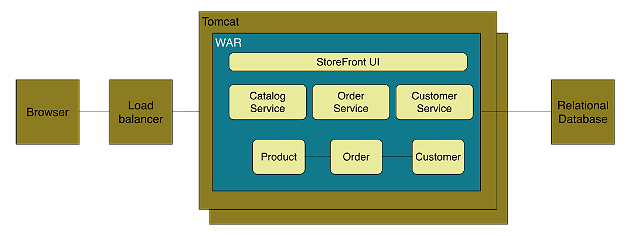
\includegraphics[width=0.8\textwidth]{figures/context-monolith-example}
\caption{Monolith Example from \cite{Richardson:2014aa}}
\label{fig:context/monolith-example}
\end{center}
\end{figure}

\subsection{Types of Monolith Architecture Style}\label{subsection:context/monolith-types}
According to \cite{Annett:2014aa}, a monolith can be of several types depending upon the viewpoint, as shown below:
\begin{enumerate}
\item Module Monolith: If all the code to realize an application share the same codebase and need to be compiled together to create a single artifact for the whole application then the architecture is Module Monolith Architecture. An example is show in figure \ref {fig:context/module-monolith-example}. The application on the left has all the code in the same codebase in the form of packages and classes without clear definition of modules and get compiled to a single artifact. However, the application on the right is developed by a number of modular codebase, each has separate codebase and can be compiled to different artifact. The modules uses the produced artifacts which is different than the earlier case where the code referenced each other directly.
\begin{figure}[H]
\begin{center}
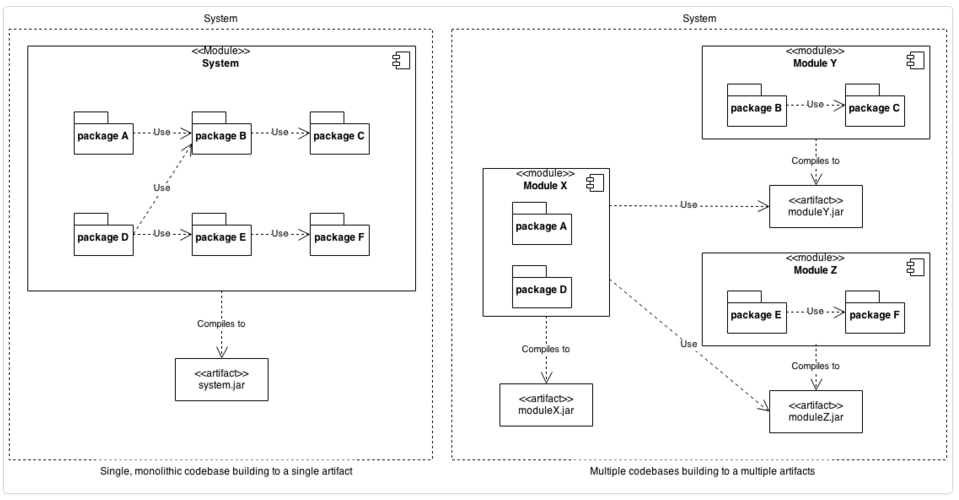
\includegraphics[width=0.8\textwidth]{figures/context-module-monolith}
\caption{Module Monolith Example from \cite{Annett:2014aa}}
\label{fig:context/module-monolith-example}
\end{center}
\end{figure}
\\
\item Allocation Monolith: An Allocation Monolith is created when all code is deployed to all the servers as a single version. This means that all the components running on the servers have the same versions at any time. The figure \ref{fig:context/allocation-monolith-example} gives an example of allocation monolith. The system on the left have same version of artifact for all the components on all the servers. It does not make any differenct whether or not the system has single codebase and artifact. However, the system on the right as shown in the figure is realized with multiple version of the artifacts in different servers at any time.
\begin{figure}[H]
\begin{center}
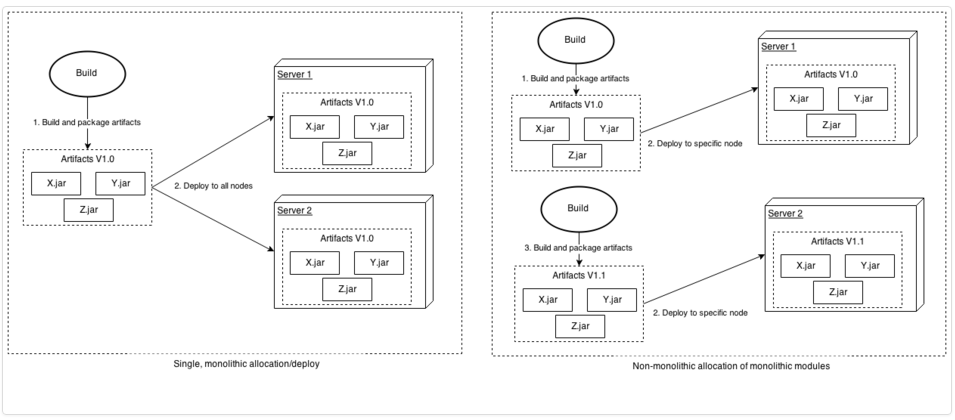
\includegraphics[width=0.8\textwidth]{figures/context-allocation-monolith}
\caption{Allocation Monolith Example from \cite{Annett:2014aa}}
\label{fig:context/allocation-monolith-example}
\end{center}
\end{figure}
\\
\item Runtime Monolith: In Runtime Monolith, the whole application is run under a single process. The left system in the figure \ref{fig:context/runtime-monolith-example} shows an example of runtime monolith where a single server process is responsible for whole application. Whereas the system on the left has allocated multiple server process to run distinct set of component artifacts of the application.
\begin{figure}[H]
\begin{center}
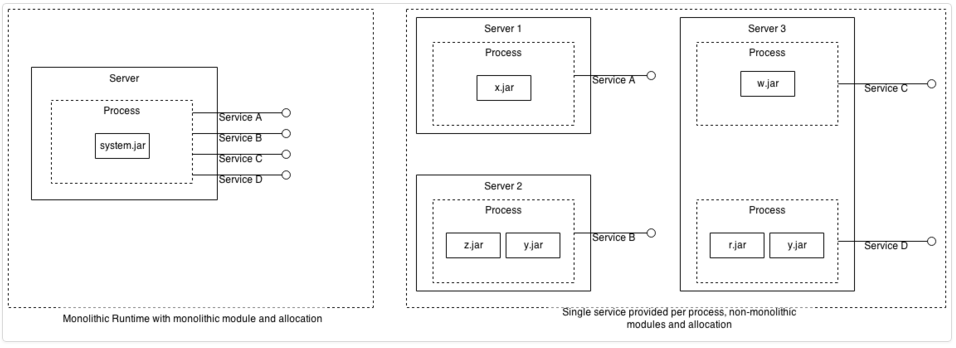
\includegraphics[width=0.8\textwidth]{figures/context-runtime-monolith}
\caption{Runtime Monolith Example from \cite{Annett:2014aa}}
\label{fig:context/runtime-monolith-example}
\end{center}
\end{figure}
\end{enumerate}

\\
\subsection{Advantages of Monolith Architecture Style}\label{subsection:context/monolith-advantages}
The Monolith architecture is appropriate for small application and has following benifits:\cite{Richardson:2014ab}\cite{Fowler:2014aa}\cite{Gupta:2015aa}\cite{Abram:2014aa}
\begin{itemize}[leftmargin=.5in]
\item It is easy to develop a monolith application since various development tools including \acrshort{IDE}s are created around the single application concept. Nevertheless, it is also easy to test the application by creating appropriate environment on the developer's machine.
\item The deployment can be simply achieved by moving the single artifact for the application to an appropriate directory in the server.
\item The scaling can be clearly and easily done by replicating the application horizontally across multiple servers behind a load balancer as shown in figure \ref{fig:context/monolith-example}
\item The different teams are working on the same codebase so sharing the functionality can be easier.
\end{itemize}
\\
\subsection{Disadvantages of Monolith Architecture Style}\label{subsection:context/monolith-disadvantages}
As the requirement grows with time, alongside as application becomes huge and the size of team increases, the monolith architecture faces many problems. Most of the advantages of monolith architecture for small application will not be valid anymore. The challenges of monolith architecture for such agile and huge context are as given below:\cite{Namiot:2014aa}\cite{Newman:2015aa}\cite{Abram:2014aa}\cite{Richardson:2014aa}\cite{Richardson:2014ab}\cite{Gupta:2015aa}
\begin{itemize}[leftmargin=.5in]
\item Limited Agility: As the whole application has single codebase, even changing a small feature to release it in production takes time. Firstly, the small change can also trigger changes to other dependent code because in huge monolith application it is very difficult to manage modularity especially when all the team members are working on the same codebase. Secondly, to deploy a small change in production, the whole application has to be deployed. Thus continuous delivery gets slower in case of monolith application. This will be more problematic when multiple changes have to be released on a daily basis. The slow pace and frequency of release will highly affect agility.
\\
\item Decrease in Productivity: It is difficult to understand the application especially for a new developer because of the size. Although it also depends upon the structure of the codebase, it will still be difficult to grasp the significance of the code when there is no hard modular boundary.Additionally, the developer can be intimidated due to need to see the whole application at once from outwards to inwards direction. Secondly, the development environment can be slow to load the whole application and at the same time the deployment will also be slow. So, in overal it will slow down the speed of understandability, execution and testing.
\\
\item Difficult Team Structure: The division of team as well as assigning tasks to the team can be tricky. Most common ways to partition teams in monolith are by technology and by geography. However, each one cannot be used in all the situations. In any case, the communication among the teams can be difficult and slow. Additionally, it is not easy to assign vertical ownership to a team from particular feature from development to relase. If something goes wrong in the deployment, there is always a confusion who should find the problem, either operations team or the last person to commit. The approprate team structure and ownership are very important for agility.
\\
\item Longterm Commitment to Technology stack: The technology to use is chosen before the development phase by analysing the requirements and the maturity of current technology at that time. All the teams in the architecture need to follow the same techonology stack. However, if the requirement changes then there can be situation when the features can be best soloved by different sets of technology. Additionally, not all the features in the application are same so cannot be treated accordingly in terms of technology as well. Nevertheless, the technology advances rapidly. So, the solution thought at the time of planning can be outdated and there can be a better solution available. In monolith application, it is very difficult to migrate to new technology stack and it can be rather painfull process.
\\
\item Limited Scalability: The scalability of monolith application can be done in either of two ways. The first way is to replicate the application along many servers and dividing the incoming request using a load balancer in front of the servers. Another approach is using the identical copies of the application in multiple servers as in previous case but partitioning the database access instead of user request. Both of these scaling approaches improves the capacity and availability of the application. However, the individual requirement regarding scaling for each component can be different but cannot be fulfilled with this approach. Also, the complexity of the monolith application remains the because we are replicating the whole application. Additionally, if there is a problem in a component the same problem can affect all the servers running the copies of the application and does not improve resilency.\cite{MacVittie:2014aa}\cite{Namiot:2014aa}
\end{itemize}
\\

\section{Microservice Architecture Style}\label{section:context/microservices_architecture_style}
With monolith, it is easy to start development. But as the system gets bigger and complicated along time, it becomes very difficult to be agile and productive. The disadvantages listed in section \ref{subsection:context/monolith-disadvantages} outweighs its advantages as the system gets old. The various qualities such as scalability, agility need to be maintained for the whole lifetime of the application and it becomes complicated by the fact that the system needs to be updated side by side because the requirements keeps coming always. In order to tackle the disadvantages, microservices architecture style is followed.\\
Microservices architecture uses the approach of decomposing an application into various dimensions as proposed by scale-cube. The detailed process of scale-cube is discussed in section \ref{section:context/microservices_architecture_style/decompostion_of_an_application}.

\subsection{Decomposition of an Application}\label{section:context/microservices_architecture_style/decompostion_of_an_application}
There are various ways to decompose an application. This section discuss two different ways of breaking down an application.
\subsubsection{Scale Cube}\label{section:context/microservices_architecture_style/decompostion_of_an_application/scale_cube}
The section \ref{subsection:context/monolith-disadvantages} specified various disadvantages related to monolith architecture style. The book \cite{Fisher:2015aa} provides a way to solve most of the discussed problems such as agility, scalability, productivity etc. It provides three dimensions of scalability as shown in figure \ref{fig:context/scale-cube} which can be applied alone or simultaneously depending upon the situation and desired goals.

\begin{figure}[H]
\begin{center}
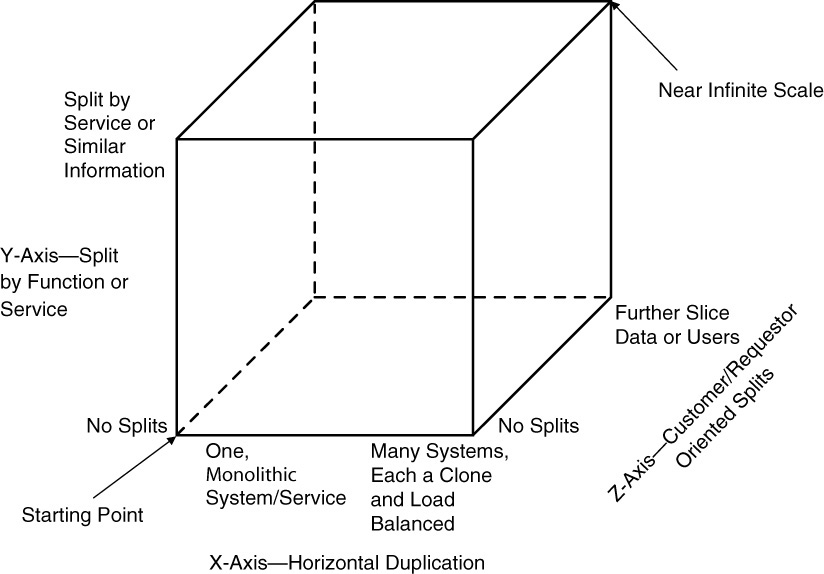
\includegraphics[width=0.6\textwidth]{figures/context-scale-cube}
\caption{Scale Cube from \cite{Fisher:2015aa}}}
\label{fig:context/scale-cube}
\end{center}
\end{figure}

\\
The scaling along each dimensions are described below. \cite{Fisher:2015aa}\cite{MacVittie:2014aa}\cite{Richardson:2014aa}
\begin{enumerate}
\item X-axis Scaling: It is done by cloning the application and data along multiple servers. A pool of requests are applied into a load balancer and the requests are deligated to any of the servers. Each of the server has the full capability of the application and full access to all the data required so in this respect it does not make any difference which server fulfills the request. Rather, it is about how many requests are fulfilled at any time. It is easy to scale along X-axis as the number of requests increases. The solution is as simple as to add additional clones. However, with this type of scaling, it is not scale with the increase in data. Moreover, it also does not scale when there are large variation in the frequency of any type of requests or there dominant requests types because all the requests are handled in an unbiased way and allocated to servers in the same way.
\\
\item Z-axis Scaling: The scaling is done by spliting the request based on certain critera or information regarding the requestor or customer affected by the request. It is different than X-axis scaling in the way that the servers are responsible for different kinds of requests. Normally, the servers have same copy of the application but some can have additional functionalies depending upon the requests expected. The Z-axis scaling helps in fault isolation and transaction scalability. Using this scaling, certain group of customers can be given added functionality or a new functionality can be tested to a small group and thus minimizing the risk.
\\
\item Y-axis Scaling: The scaling along this dimension means the spliting of the application responsibility. The separation can be done either by data, by the actions performed on the data or by combination of both. The respective ways can be referred to as resoure-oriented or service-oriented splits. While the x-axis or z-axis split were rather duplication of work along servers, the y-axis is more about specialization of work along servers. The major advantage of this scaling is that each request is scaled and handled differently according to its necessity. As the logic along with the data to be worked on are separated, developers can focus and work on small section at a time. This will increase productivity as well as agility. Additionally, a fault on a component is isolated and can be handled gracefully without affecting rest of the application. However, scaling along Y-axis can be costly compared to scaling along other dimensions.
\end{enumerate}
\subsubsection{Shared Libraries}\label{section:context/microservices_architecture_style/decompostion_of_an_application/shared_libraries}
Libraries is a standard way of sharing functionalities among various services and teams. The capability is provided by the feature of programming language. However there are various downsides to this approach. Firstly, it does not provide technology heteroginity. Next, unless the library is dynamically linked, independent scaling, deployment and maintainance cannot be achieved. So, in other cases, any small change in the library leads the redeployment of whole system. Sharing code is a form of coupling which should be avoided.

Decomposing an application in terms of composition of individual features where each feature can be scaled and deployed independently, gives various advantages along agility, performance and team organization as well. Thus, microservices uses the decomposition technique given by scale cube. A detail advantages of microservices are discussed further in section \ref{section:challanges_of_microservices_architecture/introduction/challenges}.
\subsection{Definitions}\label{section:context/microservices_architecture_style/definitions}
There are several definitions given by several pioneers and early adapters of the style.
\\
\begin{shaded}Definition 1: \cite{Richardson:2014ac} \end{shaded}
"It is the way to functionally decompose an application into a set of collaborating services, each with a set of narrow, related functions, developed and deployed independently, with its own database."

\\
\begin{shaded}Definition 2: \cite{Wootton:2014aa}\end{shaded}
"It is a style of software architecture that involves delivering systems as a set of very small, granular, independent collaborating services."


\\
\begin{shaded}Definition 3: \cite{Cockcroft:2015aa}\end{shaded}
"Microservice is a loosely coupled Service-Oriented Architecture with bounded contexts."


\\
\begin{shaded}Definition 4: \cite{Fowler:2014aa}\cite{Radchenko:2015aa}\end{shaded}
"Microservices are Service-Oriented Architecture done right."


\\
\begin{shaded}Definition 5: \cite{Fowler:2014aa}\end{shaded}
" Microservice architecture style is an approach to developing a single application as a suite of small services, each running in its own process and communicating with lightweight mechanisms, often an HTTP resource API. These services are built around business capabilities and independently deployable by fully automated deployment machinery. There is a bare minimum of centralized management of these services, which may be written in different programming languages and use different data storage technologies."
\\
As other architectural styles, microservices presents its approach by increasing cohesion and decreasing coupling. Besides that, it breaks down system along business domains following single responsibility principle into granular and autonomous services running on separate processes. Additionally, the architecture focus on the collaboration of these services using light weight mechanisms.

\section{Motivation}\label{section:context/motivation}
The various definitions presented in section highlights different key terms such as:
\begin{enumerate}
\item collaborating services
\item developed and deployed independently
\item build around business capabilities
\item small, granular services
\end{enumerate}
These concepts are very important to be understood in order to approach microservices correctly and effectively. The first two terms relate to runtime operational qualities of microservices whereas the next two address modeling qualities. With that consideration, it indicates that the definitions given are complete which focus on both aspects of any software applications. \\
However, if attempt is made to have clear indepth understanding of each of the key terms then various questions can be raised without appropriate answers. The various questions related to modeling and operations are listed in the table \ref{tab:context/microservices_architecture_style/various_questions_related_to_microservices}.
\begin{table}[H]
  \centering
  \begin{adjustbox}{max width=\textwidth}
  \begin{tabular}{*{14}{|c}|}%%{|c|c|}
  \hline
  \# & Questions & Type\\
  \hline
  \hline
   1 & How small should be size of microservices? &  Modeling  \\ \hline
   2 & How does the collaboration among services happen? & Operation  \\ \hline
   3 & How to deploy and maintain independently when there are dependencies among services?& Operation   \\ \hline
   4 & How to map microservices from business capabilities? & Modeling\\ \hline
   5 & What are the challenges need to be tackled and how to? & Operation\\ \hline \hline
   \end{tabular}
\end{adjustbox}
  \caption{Various Questions related to Microservices}
  \label{tab:context/microservices_architecture_style/various_questions_related_to_microservices}
\end{table}
Without clear answer to these questions, it is difficult to say that the definitions presented in section are complete and enough to follow the microservices architecture. The process of creating microservices is not clearly documented. There is no enough research papers defining a thorough process of modeling and operating microservices. Additionally, a lot of industries such as amazon, netflix etc are following this architecture but it is not clear about the process they are using to define and implement microservices. The purpose of the research is to have a clear understanding about the process of designing microservices by focusing on following questions.
\begin{shaded}
\textbf{Research Questions}\label{list:introduction/research_questions}
\end{shaded}
\begin{enumerate}
\item How are boundary and size of microservices defined?
\item How business capabilities are mapped to define microservices?
\item What are the best practices to tackle challenges introduced by microservices?
    \begin{enumerate}
    \item How does the collaboration among services happen?
    \item How to deploy and maintain independently when there are dependencies among services?
    \item How to monitor microservices?
    \end{enumerate}
\end{enumerate}
\section{Approach}\label{section:context/approach}
The various definitions in section \ref{section:context/microservices_architecture_style/definitions} show that the authors have their own way of interpretation of microservices but at the same time agree upon some basic concepts regarding the architecture. However, each definition can be used to understand different aspect of the microservices. A distinct set of keywords can be identified which represents different aspects pointed by the authors and various concepts they agree. Moreover, the table lists important keywords.

\begin{table}[H]
  \centering
  \begin{adjustbox}{max width=\textwidth}
  \begin{tabular}{*{14}{|c}|}%%{|c|c|c|c|c|c|}
  \hline
  \# & keywords & size & Quality of good microservice & communication & process to model microservices\\
  \hline
  \hline
   1 & Collaborating Services                                       &   &   & \checkmark &  \\ \hline
   2 & Communicating with lightweight mechanism like http           &   &   & \checkmark &  \\ \hline
   3 & Loosely coupled, related functions                           &   & \checkmark  & \checkmark &   \\ \hline
   4 & Developed and deployed independently       &  &   &  & \checkmark \\ \hline
   5 & Own database                                 &  & \checkmark &  & \checkmark \\ \hline
   6 & Different database technologies         &  &  &  & \checkmark \\ \hline
   7 & Service Oriented Architecture  & & \checkmark &  & \checkmark \\ \hline
   8 & Bounded Context  & \checkmark & \checkmark &  & \checkmark \\ \hline
   9 & Build around Business Capabilities  & \checkmark & \checkmark &  &\checkmark \\ \hline
   10 & Different Programming Languages & &  & & \checkmark \\ \hline
   \hline
   \end{tabular}
\end{adjustbox}
  \caption{Keywords extracted from various definitions of Microservice}
  \label{tab:context/microservices_architecture_style/keywords_extracted_from_various_definitions_of_microservice}
\end{table}
These keywords provide us some hint regarding various topics of discussion related to microservices, which are listed in columns. Finally, answering various questions around these keywords can be the \textbf{first approach} to understand the topics shown in columns such as size, quality of microservices etc.
\\
The \textbf{next approach} to look around the architecture process is to understand various drivers. According to , the important drivers which clarify the architecture are: \cite{Brown:2015aa} \label{list:introduction/drivers}
\begin{enumerate}
\item \textbf{Quality Attributes}\\
The non-functional requirements have high impact on the resulting architecture. It is important to consider various quality attributes to define the process of architecture.
\item \textbf{Constraints}\\
There are always limitations or disadvantages faced by any architecture however the better knowledge is useful in the process of explaining the architecture with satisfaction.
\item \textbf{Principles}\\
The various principles provides a consistent approaches to tackle various limitations. They are the keys to define guidelines.
\end{enumerate}
So, in order to define the process of modeling microservices, the key aspects related to \textbf{quality attributes}, \textbf{constraints} and \textbf{principles} will be studied thoroughly.
\\
\\
Considering both the table \ref{tab:context/microservices_architecture_style/keywords_extracted_from_various_definitions_of_microservice} and list \ref{list:introduction/drivers}, the approach to be used to define the guidelines will be to look deep into various quality attributes influencing microservices architecture. Then, the process of identifying or modeling individual microservices from problem domain will be defined. At first, the research is performed based on various research papers. Then, the approach used by industry adopting microservices architecture will be studied in order to answer the research questions. The study will be performed on SAP Hybris.
Finally, the various constraints or challenges which affects microservices will be identified. 
The results of previous research will be mapped into a form of various principles and these principles will ultimately provide sufficient ground to create guidelines to create microservices architecture.



